\documentclass[border=0.1cm]{standalone}
\usepackage{tikz}
\usetikzlibrary{arrows, arrows.meta}

\tikzset{
    larrow/.style={
        >={Triangle[left,length=6pt,width=4pt]},
        shorten >= 4pt, shorten <= 4pt,
        semithick,
        ->
    }
}
\newcommand{\halfedge}[2]
{
    \draw[larrow, transform canvas={yshift=1.5pt}] (#1) -- (#2);
    \draw[larrow, transform canvas={yshift=-1.5pt}] (#2) -- (#1);
}

\begin{document}
    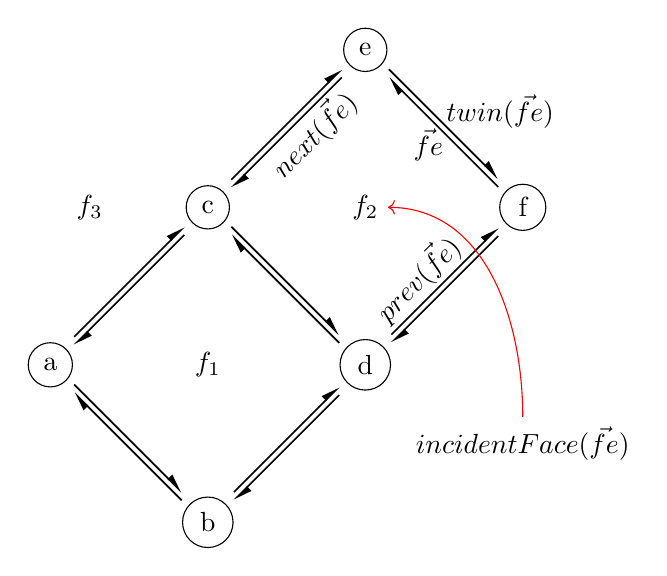
\begin{tikzpicture}
        \tikzstyle{node1}=[draw,shape=circle,color=black,fill=white, minimum size=5pt]
        \tikzstyle{node2}=[color=black,fill=white]

        \node[node1] (A) at (0,2)   {a};
        \node[node1] (B) at (2,0)   {b};
        \node[node1] (C) at (2,4)   {c};
        \node[node1] (D) at (4,2)   {d};
        \node[node1] (E) at (4,6)   {e};
        \node[node1] (F) at (6,4)   {f};

        \halfedge{A}{C}
        \halfedge{A}{B}
        \halfedge{C}{D}
        \halfedge{B}{D}
        \draw[larrow, transform canvas={yshift=1.5pt}]  (E) -- (F) node[pos=0.4, xshift=2.5em] {$twin(\vec{fe})$};
        \draw[larrow, transform canvas={yshift=-1.5pt}] (F) -- (E) node[pos=0.4, xshift=-1em] {$\vec{fe}$};
        \draw[larrow, transform canvas={yshift=1.5pt}]  (C) -- (E);
        \draw[larrow, transform canvas={yshift=-1.5pt}] (E) -- (C) node[pos=0.4, rotate=45, yshift=-0.75em] {$next(\vec{fe})$};
        \draw[larrow, transform canvas={yshift=1.5pt}]  (D) -- (F) node[pos=0.4, rotate=45, yshift=0.75em] {$prev(\vec{fe})$};
        \draw[larrow, transform canvas={yshift=-1.5pt}] (F) -- (D);
        \node[node2] (P) at (6,1) {$incidentFace(\vec{fe})$};
        \node[node2] (S) at (0.5,4) {$f_3$};
        \node[node2] (Q) at (4,4) {$f_2$};
        \node[node2] (R) at (2,2) {$f_1$};
        \draw[->, red] (P) to [out=90,in=0] (Q);
    \end{tikzpicture}
\end{document}
